%-----------------------------------------------------------------------------------------------
\makeatletter
\immediate\write18{datelog > \jobname.info} % site script for $(date '+%Y-%m-%d %Hh%Mm%Ss')
\makeatother
%-----------------------------------------------------------------------------------------------
%-----------------------------------------------------------------------------------------------
\usetheme{Copenhagen}
\usepackage{beamercolorthemeCNThermSci2}
\usefonttheme{serif}
%-----------------------------------------------------------------------------------------------

%-----------------------------------------------------------------------------------------------
%-----------------------------------------------------------------------------------------------
\usetheme{Copenhagen}
\usepackage{beamercolorthemeUTF2}
\usefonttheme{serif}
%-----------------------------------------------------------------------------------------------
\usepackage[utf8]{inputenc}
\usepackage[greek,french,english,brazil]{babel} % last becomes the active one
\usepackage{pslatex}
\usepackage{amssymb,amsmath}
\usepackage{soul}
\usepackage[squaren,Gray,cdot]{SIunits}
\usepackage[nice]{nicefrac}
\usepackage{tikz}
\usepackage{amscd}
\usepackage{stmaryrd}
\usepackage{scalerel}
\usepackage{xspace}
%-----------------------------------------------------------------------------------------------


%-----------------------------------------------------------------------------------------------
%-----------------------------------------------------------------------------------------------
% Mathematical
%-----------------------------------------------------------------------------------------------
\newcommand{\vet}[1]{\underline{{#1}}}
\newcommand{\mat}[1]{\underline{\underline{{#1}}}}
\newcommand{\cub}[1]{\underline{\underline{\underline{{#1}}}}}
\newcommand{\eqdef}{{\ensuremath\stackrel{\text{\tiny def}}{=}}}
%-----------------------------------------------------------------------------------------------
% Linguistic
%-----------------------------------------------------------------------------------------------
\newcommand{\GRtxt}[1]{\begin{otherlanguage}{greek}{{#1}}\end{otherlanguage}}
\newcommand{\FRtxt}[1]{\begin{otherlanguage}{french}{{#1}}\end{otherlanguage}}
%-----------------------------------------------------------------------------------------------
% Presentation
%-----------------------------------------------------------------------------------------------
\newcommand{\BkgImgH}[1]{% Places an image centered on the slide background filling the height
    \usebackgroundtemplate{\parbox{\paperwidth}{%
        \vspace*{1sp}\centering\includegraphics[height=\paperheight]{{#1}}
}}}
\newcommand{\BkgImgW}[1]{% Places an image centered on the slide background filling the width
    \usebackgroundtemplate{\parbox{\paperwidth}{%
        \vspace*{1sp}\centering\includegraphics[width=\paperwidth]{{#1}}
}}}
\newcommand{\ArtEndH}[3]{% Transitions to plain image (last) slide: #1:prefix #2,#3:extensions
    \BkgImgH{root/../art/#1.#2}
    \frame<handout:0>[plain]{%
        \transdissolve\vspace*{72mm}\color{white}\scriptsize\bf\input{root/../art/#1.#3}}
    \usebackgroundtemplate{\mbox{~}}
}
\newcommand{\ArtEndW}[3]{% Transitions to plain image (last) slide: #1:prefix #2,#3:extensions
    \BkgImgW{root/../art/#1.#2}
    \frame<handout:0>[plain]{%
        \transdissolve\vspace*{72mm}\color{white}\scriptsize\bf\input{root/../art/#1.#3}}
    \usebackgroundtemplate{\mbox{~}}
}
\newcommand{\ImgColW}[3]{% Inserts a full-width image in a column
    \includegraphics[width=\columnwidth]{root/../art/#1.#2}\\[-0.5\baselineskip]
    \parbox{\columnwidth}{\tiny\hfill\scalebox{0.85}{\input{root/../art/#1.#3}}}
}
\newcommand{\txtpic}[1]{%
    \fcolorbox{lightgray}{white!90!black}{{#1}} 
}
%-----------------------------------------------------------------------------------------------


%-----------------------------------------------------------------------------------------------
\newcommand{\VPMS}{{\ensuremath V_{\mathrm{PMS}}}}
\newcommand{\VPMI}{{\ensuremath V_{\mathrm{PMI}}}}
%-----------------------------------------------------------------------------------------------
\title{An Inertial Air-standard Finite-time Heat\\ Addition Otto Engine Model}
\subtitle{ENC-2020-0067}
\author{F.~M.~Moreira and Prof.~C.~Naaktgeboren, PhD}
\date{{\scriptsize\tt%
    
\includegraphics[height=6.0mm]{root/00-res/cc/by-nc-nd-88x31.pdf}\\[\smallskipamount]
    https://github.com/CNThermSci/ApplThermSci\\
    Compiled on \input{\jobname.info}
}}
%-----------------------------------------------------------------------------------------------
\begin{document}
%-----------------------------------------------------------------------------------------------
\logo{%
    \parbox{158mm}{% There's a 1mm gap on each side of the 160mm x 90mm slide logo line
        \mode<beamer>{
            
\includegraphics[height=6.0mm]{root/00-res/UTFPR/UTFPR-logo-D.pdf}\hfill%
            
\includegraphics[height=9.0mm]{root/00-res/logo/CNThermSci-logo-A.pdf}%
        }
        \mode<handout>{
            
\includegraphics[height=6.0mm]{root/00-res/UTFPR/UTFPR-logo-W.pdf}\hfill%
            
\includegraphics[height=9.0mm]{root/00-res/logo/CNThermSci-logo-W.pdf}%
        }
    }
} % The (delineated, alpha), or washed-out logos
%-----------------------------------------------------------------------------------------------
\frame{\titlepage}
\frame{\tableofcontents}
%-----------------------------------------------------------------------------------------------

%-----------------------------------------------------------------------------------------------
\section{iFTHA Modeling}
%-----------------------------------------------------------------------------------------------

%-----------------------------------------------------------------------------------------------
\subsection{Introduction}
%-----------------------------------------------------------------------------------------------

    % !j 96 -i8
    %-------------------------------------------------------------------------------------------
    \begin{frame}{iFTHA}\vspace*{-2em}
        \uncover<1->{The work proposes a}\vspace*\medskipamount
        \begin{itemize}
            \item<1->  fairly simple \alert{coupled dynamic-thermodynamic} engine model, i.e.,
            \item<1->  an \alert{inertial}, \alert{air-standard}, Otto model with:
            \item<1->  \alert{finite-time} heat release,
            \item<1->  basic \alert{engine parameters}, and
            \item<1->  \alert{piston}, \alert{rod}, \alert{crank}, and \alert{flywheel}
                inertias.
        \end{itemize}
    \end{frame}
    %-------------------------------------------------------------------------------------------

    % !j 96 -i8
    %-------------------------------------------------------------------------------------------
    \begin{frame}{Motivation}\vspace*{-2em}
        \uncover<1->{Somewhat recently published$^\dagger$ FTHA model:}\vspace*\medskipamount
        \begin{itemize}
            \item<1->  \alert{Air-standard reversible},
            \item<1->  \alert{finite-time} heat release,
            \item<1->  Otto engine (spark-ignited) model:
            \item<1->  \alert{minimal-complexity}, \alert{pure-substance} model
            \item<1->  accounting for \alert{simultaneous heat+work} interactions.
        \end{itemize}\vspace*\medskipamount
        {\scriptsize
        $^\dagger$~Naaktgeboren, C. Int.~J.~Mech.~Eng.~Educ., 45(2), 2017.}
    \end{frame}
    %-------------------------------------------------------------------------------------------

    % !j 96 -i8
    %-------------------------------------------------------------------------------------------
    \begin{frame}\vspace*{-2em}
        \begin{center}
            \noindent\hspace*{-4.5mm}%
            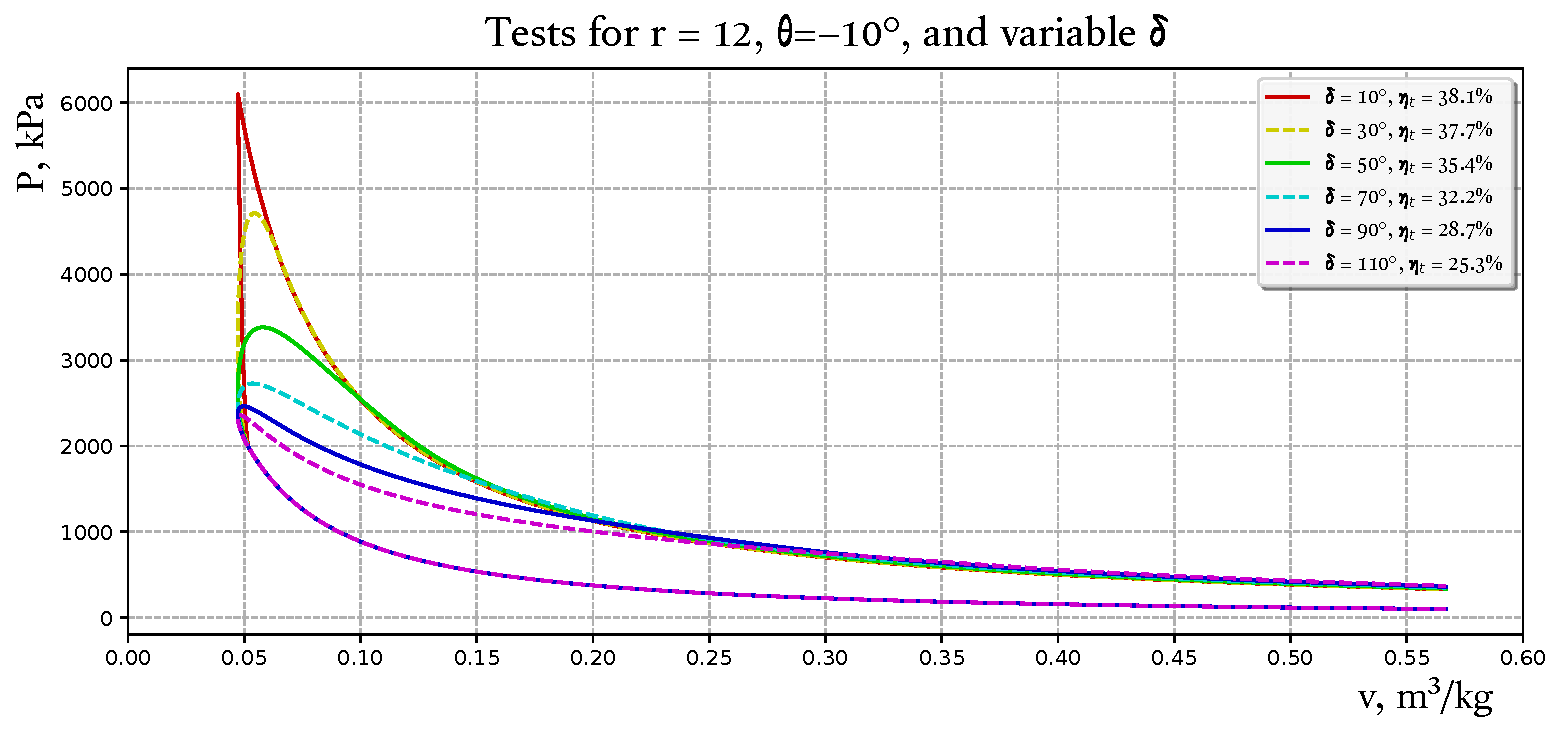
\includegraphics[height=70.0mm]{01-FTHA/fig/test_r=12,0_speed-P.pdf}
        \end{center}
    \end{frame}
    %-------------------------------------------------------------------------------------------

%-----------------------------------------------------------------------------------------------
\subsection{Thermodynamic Modeling}
%-----------------------------------------------------------------------------------------------

    % !j 96 -i8
    %-------------------------------------------------------------------------------------------
    \begin{frame}{Title}{Subtitle}\vspace*{-2em}
        \uncover<1->{Some text:}
        \begin{itemize}
            \item<2->  A \alert{relevant} item;
            \item<3->  Another \alert{important} point;
        \end{itemize}
    \end{frame}
    %-------------------------------------------------------------------------------------------

%-----------------------------------------------------------------------------------------------
\subsection{Dynamic Modeling}
%-----------------------------------------------------------------------------------------------

    % !j 96 -i8
    %-------------------------------------------------------------------------------------------
    \begin{frame}{Title}{Subtitle}\vspace*{-2em}
        \uncover<1->{Some text:}
        \begin{itemize}
            \item<2->  A \alert{relevant} item;
            \item<3->  Another \alert{important} point;
        \end{itemize}
    \end{frame}
    %-------------------------------------------------------------------------------------------

%-----------------------------------------------------------------------------------------------
\section{iFTHA Results}
%-----------------------------------------------------------------------------------------------

%-----------------------------------------------------------------------------------------------
\subsection{Validation Results}
%-----------------------------------------------------------------------------------------------

    % !j 96 -i8
    %-------------------------------------------------------------------------------------------
    \begin{frame}{Title}{Subtitle}\vspace*{-2em}
        \uncover<1->{Some text:}
        \begin{itemize}
            \item<2->  A \alert{relevant} item;
            \item<3->  Another \alert{important} point;
        \end{itemize}
    \end{frame}
    %-------------------------------------------------------------------------------------------

%-----------------------------------------------------------------------------------------------
\subsection{Case Study Results}
%-----------------------------------------------------------------------------------------------

    % !j 96 -i8
    %-------------------------------------------------------------------------------------------
    \begin{frame}{Single-Cycle No-load Acceleration}{Subtitle}\vspace*{-2em}
        \uncover<1->{Some text:}
        \begin{itemize}
            \item<2->  A \alert{relevant} item;
            \item<3->  Another \alert{important} point;
        \end{itemize}
    \end{frame}
    %-------------------------------------------------------------------------------------------

    % !j 96 -i8
    %-------------------------------------------------------------------------------------------
    \begin{frame}{Multiple-Cycle No-load Acceleration}{Subtitle}\vspace*{-2em}
        \uncover<1->{Some text:}
        \begin{itemize}
            \item<2->  A \alert{relevant} item;
            \item<3->  Another \alert{important} point;
        \end{itemize}
    \end{frame}
    %-------------------------------------------------------------------------------------------

%-----------------------------------------------------------------------------------------------
\section{Conclusions}
%-----------------------------------------------------------------------------------------------

    % !j 96 -i8
    %-------------------------------------------------------------------------------------------
    \begin{frame}{Title}{Subtitle}\vspace*{-2em}
        \uncover<1->{Some text:}
        \begin{itemize}
            \item<2->  A \alert{relevant} item;
            \item<3->  Another \alert{important} point;
        \end{itemize}
    \end{frame}
    %-------------------------------------------------------------------------------------------

%-----------------------------------------------------------------------------------------------
% End splash screen
%-----------------------------------------------------------------------------------------------

    % Finishes with stunning image, with credit
    \ArtEndW{pexels-alexandre-saraiva-carniato-2309922}{jpg}{txt}

%-----------------------------------------------------------------------------------------------
\end{document}
%-----------------------------------------------------------------------------------------------

